\documentclass[dvipdfmx]{article}
\usepackage[dvipdfmx]{graphicx}
\usepackage{amsmath, amssymb}
\usepackage{mathtools}
\usepackage{here}
\begin{document}
\title{Weekly Report}
\author{Riku Gondow}
\maketitle
\section{Progress}
\begin{itemize}
    \item Try to implement LSTM-CNN Ensemble method with 30-subjects dataset.\cite{lstm}
    \begin{itemize}
        \item I've been working on fixing bugs for a while.
    \end{itemize}

    \item (Contact with Mr.Ohba about WFIoT2022, and adjust the shift schedule.)
\end{itemize}

\begin{figure}[H]
    \begin{center}
    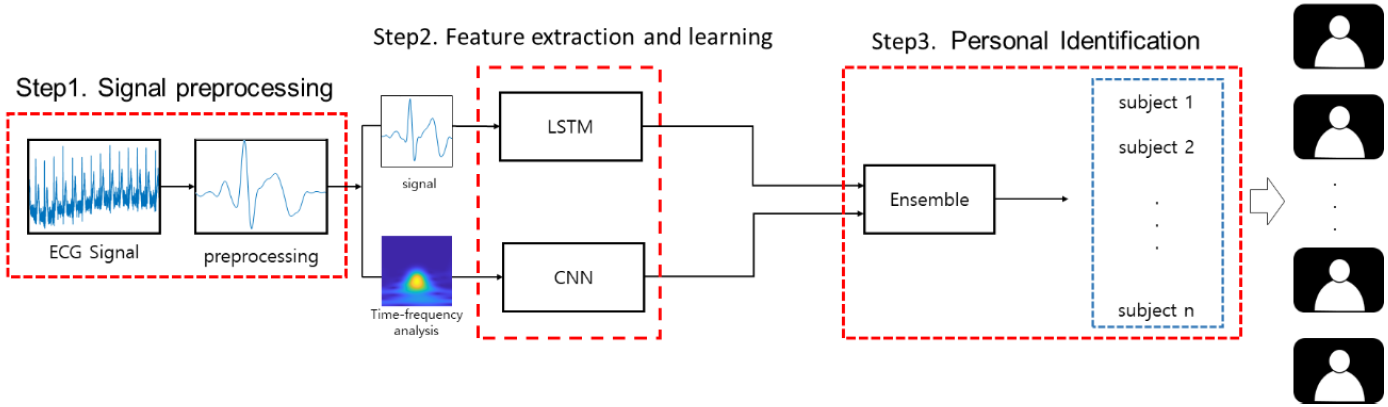
\includegraphics[width=\linewidth]{./img/LSTM-CNN.png}
    \end{center}
    \caption{LSTM-CNN Ensemble method}
\end{figure}

\section{Next Plan}
\begin{itemize}
    \item Ask seniors about the bugs
    \item Continue to implement and evaluate LSTM-CNN Ensemble method
    \item Check the ECG reconstruction paper\cite{ECG} and the source code that Yamamoto-san will share with me.
\end{itemize}

\begin{thebibliography}{99}
\bibitem{lstm} Lee, Jin-A., and Keun-Chang Kwak. "Personal Identification Using an Ensemble Approach of 1D-LSTM and 2D-CNN with Electrocardiogram Signals." Applied Sciences 12.5 2022: 2692.
\bibitem{ECG} K. Yamamoto, R. Hiromatsu and T. Ohtsuki, "ECG Signal Reconstruction via Doppler Sensor by Hybrid Deep Learning Model With CNN and LSTM," in IEEE Access, vol. 8, pp. 130551-130560, 2020, doi: 10.1109/ACCESS.2020.3009266.
\end{thebibliography}
\end{document}